\documentclass{article}
\usepackage[T1]{fontenc}
\usepackage[utf8]{inputenc}
\usepackage[swedish]{babel}
\usepackage{amsmath, amssymb, mathtools}
\usepackage{enumitem}
\usepackage{siunitx}
\usepackage{listings}
\usepackage{comment}
\usepackage{tikz, pgfplots}
\usepackage{afterpage}
\usepackage{booktabs}

\makeatletter
\def\fps@figure{hbtp}
\def\fps@table{hbtp}
\makeatother

\pgfplotsset{compat=newest}
\sisetup{
	round-mode      = places,
	round-precision = 3
	}

\lstset{
	breaklines=true,
	postbreak=\mbox{\textcolor{red}{$\hookrightarrow$}\space},
	}

\DeclareMathOperator\Poisson{Pois}
\DeclareMathOperator\GammaDist{Gamma}
\DeclareMathOperator\Normal{Normal}
\DeclareMathOperator\NegBin{Neg-Bin}
\DeclareMathOperator\Uniform{Uniform}
\newcommand{\size}[1]{\lvert #1 \rvert}

\title{Third Assignment in MVE550}
\author{Axel Forsman, Jonas Lauri}

\begin{document}
% \maketitle

\section{Question 1}
\begin{enumerate}[label=(\alph*)]
	\item Fin.
\end{enumerate}

\subsection{(a)}
$(N_A)_{A \subseteq \mathbb R^2}$ is a spatial Poisson process
with parameter $\lambda = 36$.
Let $A \coloneqq [0.2, 0.6] \times [0.2, 0.6] \subseteq \mathbb R^2$.
Then $N_A$ has a Poisson distribution with parameter $\lambda \lvert A \rvert$.
Whence we get
$$ \mathbb P(N_A \ge 6) = 1 - \mathbb P(N_A \le 5) = 1 - \Poisson(5; 36 \cdot 0.4^2)
\approx \num{0.5150434} $$

\subsection{(b)}
\begin{center}
	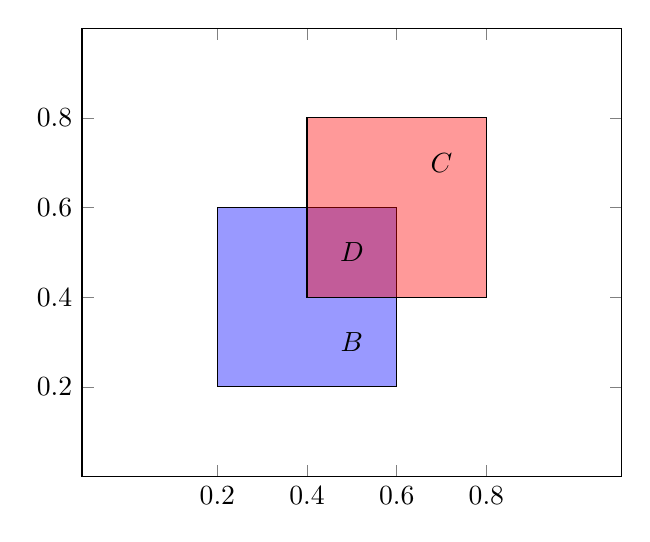
\begin{tikzpicture}
		\begin{axis}[xmin = 0, xmax = 1, ymin=0, ymax = 1, axis equal,
			xtick = {0.2, 0.4, 0.6, 0.8}, ytick = {0.2, 0.4, 0.6, 0.8},
			clip = false]
			\fill[blue, fill opacity=0.4, draw=black] (0.2, 0.2) rectangle (0.6, 0.6);
			\fill[red, fill opacity=0.4, draw=black] (0.8, 0.8) rectangle (0.4, 0.4);
			\node at (0.5, 0.3) {$B$};
			\node at (0.7, 0.7) {$C$};
			\node at (0.5, 0.5) {$D$};
		\end{axis}
	\end{tikzpicture}
\end{center}

Let $B \coloneqq A \setminus D, C \coloneqq A \setminus D, D \coloneqq [0.4, 0.6]^2$.
Then
\begin{align*}
	\mathbb P(N_{B \cup D = 4}, N_{C \cup D = 4}) &= \sum_{k=0}^4 \mathbb P(N_D = k) \underbrace{\mathbb P(N_{B \cup D} = 4, N_{C \cup D} = 4 \mid N_D = k)}_{\mathbb P(N_B = 4 - k, N_C = 4 - k)} \\
												  &= \sum_{k=0}^4 \mathbb P(N_D = k) \mathbb P(N_B = 4 - k) \mathbb P(N_C = 4 - k) \\
												  &= \sum_{k=0}^4 \Poisson(k; \lambda \size{D}) \Poisson(4 - k; \lambda \size{B})^2
												  \approx \num{0.023902}
\end{align*}
where we have used that $N_B, N_C$ are independent since $B, C$ are disjoint.

\subsection{(c)}
Since conditional on the number of points in $A \coloneqq [0, 1]^2$,
the positions of the points are uniformly distributed in $A$,
we can simulate such a process using
\begin{lstlisting}[language = R]
N <- rpois(1, lambda * 1^2)
list(x = runif(N, 0, 1), y = runif(N, 0, 1))
\end{lstlisting}
One such example simulation is shown in figure~\ref{fig:c_sim}.

\begin{figure}
	\centering
	% Created by tikzDevice version 0.12.3 on 2019-12-19 22:07:12
% !TEX encoding = UTF-8 Unicode
\begin{tikzpicture}[x=1pt,y=1pt]
\definecolor{fillColor}{RGB}{255,255,255}
\path[use as bounding box,fill=fillColor,fill opacity=0.00] (0,0) rectangle (289.08,289.08);
\begin{scope}
\path[clip] ( 67.20, 61.20) rectangle (245.88,239.88);
\definecolor{drawColor}{RGB}{0,0,0}

\path[draw=drawColor,line width= 0.4pt,line join=round,line cap=round] ( 79.52,203.63) --
	( 82.55,198.38) --
	( 76.49,198.38) --
	( 79.52,203.63);

\path[draw=drawColor,line width= 0.4pt,line join=round,line cap=round] (175.57,171.63) --
	(178.60,166.38) --
	(172.54,166.38) --
	(175.57,171.63);

\path[draw=drawColor,line width= 0.4pt,line join=round,line cap=round] (237.38,172.85) --
	(240.41,167.60) --
	(234.35,167.60) --
	(237.38,172.85);

\path[draw=drawColor,line width= 0.4pt,line join=round,line cap=round] (210.39,147.15) --
	(213.42,141.90) --
	(207.36,141.90) --
	(210.39,147.15);

\path[draw=drawColor,line width= 0.4pt,line join=round,line cap=round] (110.90,129.00) --
	(113.93,123.75) --
	(107.87,123.75) --
	(110.90,129.00);

\path[draw=drawColor,line width= 0.4pt,line join=round,line cap=round] (154.71,135.60) --
	(157.74,130.36) --
	(151.68,130.36) --
	(154.71,135.60);

\path[draw=drawColor,line width= 0.4pt,line join=round,line cap=round] ( 97.72,178.77) --
	(100.75,173.52) --
	( 94.69,173.52) --
	( 97.72,178.77);

\path[draw=drawColor,line width= 0.4pt,line join=round,line cap=round] (161.42, 93.90) --
	(164.45, 88.65) --
	(158.39, 88.65) --
	(161.42, 93.90);

\path[draw=drawColor,line width= 0.4pt,line join=round,line cap=round] (171.57,224.93) --
	(174.60,219.68) --
	(168.54,219.68) --
	(171.57,224.93);

\path[draw=drawColor,line width= 0.4pt,line join=round,line cap=round] (194.13,226.44) --
	(197.16,221.19) --
	(191.10,221.19) --
	(194.13,226.44);

\path[draw=drawColor,line width= 0.4pt,line join=round,line cap=round] (121.23,226.52) --
	(124.26,221.27) --
	(118.20,221.27) --
	(121.23,226.52);

\path[draw=drawColor,line width= 0.4pt,line join=round,line cap=round] (173.27, 79.57) --
	(176.30, 74.32) --
	(170.24, 74.32) --
	(173.27, 79.57);

\path[draw=drawColor,line width= 0.4pt,line join=round,line cap=round] (222.15,145.99) --
	(225.18,140.74) --
	(219.12,140.74) --
	(222.15,145.99);

\path[draw=drawColor,line width= 0.4pt,line join=round,line cap=round] (185.80, 78.45) --
	(188.83, 73.20) --
	(182.77, 73.20) --
	(185.80, 78.45);

\path[draw=drawColor,line width= 0.4pt,line join=round,line cap=round] (204.30, 73.37) --
	(207.33, 68.13) --
	(201.27, 68.13) --
	(204.30, 73.37);

\path[draw=drawColor,line width= 0.4pt,line join=round,line cap=round] (189.18,150.21) --
	(192.21,144.96) --
	(186.15,144.96) --
	(189.18,150.21);

\path[draw=drawColor,line width= 0.4pt,line join=round,line cap=round] (148.49,134.06) --
	(151.52,128.81) --
	(145.46,128.81) --
	(148.49,134.06);

\path[draw=drawColor,line width= 0.4pt,line join=round,line cap=round] (115.08, 82.93) --
	(118.11, 77.68) --
	(112.04, 77.68) --
	(115.08, 82.93);

\path[draw=drawColor,line width= 0.4pt,line join=round,line cap=round] (173.21,199.38) --
	(176.24,194.13) --
	(170.18,194.13) --
	(173.21,199.38);

\path[draw=drawColor,line width= 0.4pt,line join=round,line cap=round] (167.74,112.36) --
	(170.77,107.12) --
	(164.71,107.12) --
	(167.74,112.36);

\path[draw=drawColor,line width= 0.4pt,line join=round,line cap=round] (110.83,185.21) --
	(113.86,179.96) --
	(107.80,179.96) --
	(110.83,185.21);

\path[draw=drawColor,line width= 0.4pt,line join=round,line cap=round] (115.54,136.11) --
	(118.57,130.86) --
	(112.51,130.86) --
	(115.54,136.11);

\path[draw=drawColor,line width= 0.4pt,line join=round,line cap=round] ( 91.68, 75.26) --
	( 94.71, 70.01) --
	( 88.65, 70.01) --
	( 91.68, 75.26);

\path[draw=drawColor,line width= 0.4pt,line join=round,line cap=round] (233.80,220.33) --
	(236.83,215.08) --
	(230.77,215.08) --
	(233.80,220.33);

\path[draw=drawColor,line width= 0.4pt,line join=round,line cap=round] (126.67, 95.01) --
	(129.70, 89.76) --
	(123.64, 89.76) --
	(126.67, 95.01);

\path[draw=drawColor,line width= 0.4pt,line join=round,line cap=round] (129.28,175.16) --
	(132.31,169.91) --
	(126.25,169.91) --
	(129.28,175.16);

\path[draw=drawColor,line width= 0.4pt,line join=round,line cap=round] ( 74.42,201.30) --
	( 77.45,196.05) --
	( 71.39,196.05) --
	( 74.42,201.30);

\path[draw=drawColor,line width= 0.4pt,line join=round,line cap=round] (110.58,158.63) --
	(113.61,153.38) --
	(107.55,153.38) --
	(110.58,158.63);

\path[draw=drawColor,line width= 0.4pt,line join=round,line cap=round] (147.70,141.72) --
	(150.73,136.47) --
	(144.67,136.47) --
	(147.70,141.72);

\path[draw=drawColor,line width= 0.4pt,line join=round,line cap=round] ( 94.82,228.55) --
	( 97.85,223.30) --
	( 91.79,223.30) --
	( 94.82,228.55);

\path[draw=drawColor,line width= 0.4pt,line join=round,line cap=round] (202.26,100.34) --
	(205.29, 95.09) --
	(199.23, 95.09) --
	(202.26,100.34);

\path[draw=drawColor,line width= 0.4pt,line join=round,line cap=round] (235.79,168.18) --
	(238.82,162.93) --
	(232.76,162.93) --
	(235.79,168.18);

\path[draw=drawColor,line width= 0.4pt,line join=round,line cap=round] (206.44,154.74) --
	(209.47,149.49) --
	(203.40,149.49) --
	(206.44,154.74);

\path[draw=drawColor,line width= 0.4pt,line join=round,line cap=round] ( 86.17,101.67) --
	( 89.20, 96.43) --
	( 83.14, 96.43) --
	( 86.17,101.67);

\path[draw=drawColor,line width= 0.4pt,line join=round,line cap=round] (220.61,221.41) --
	(223.64,216.16) --
	(217.58,216.16) --
	(220.61,221.41);

\path[draw=drawColor,line width= 0.4pt,line join=round,line cap=round] ( 90.41,202.85) --
	( 93.44,197.60) --
	( 87.38,197.60) --
	( 90.41,202.85);
\end{scope}
\begin{scope}
\path[clip] (  0.00,  0.00) rectangle (289.08,289.08);
\definecolor{drawColor}{RGB}{0,0,0}

\path[draw=drawColor,line width= 0.4pt,line join=round,line cap=round] ( 73.82, 61.20) -- (239.26, 61.20);

\path[draw=drawColor,line width= 0.4pt,line join=round,line cap=round] ( 73.82, 61.20) -- ( 73.82, 55.20);

\path[draw=drawColor,line width= 0.4pt,line join=round,line cap=round] (106.91, 61.20) -- (106.91, 55.20);

\path[draw=drawColor,line width= 0.4pt,line join=round,line cap=round] (140.00, 61.20) -- (140.00, 55.20);

\path[draw=drawColor,line width= 0.4pt,line join=round,line cap=round] (173.08, 61.20) -- (173.08, 55.20);

\path[draw=drawColor,line width= 0.4pt,line join=round,line cap=round] (206.17, 61.20) -- (206.17, 55.20);

\path[draw=drawColor,line width= 0.4pt,line join=round,line cap=round] (239.26, 61.20) -- (239.26, 55.20);

\node[text=drawColor,anchor=base,inner sep=0pt, outer sep=0pt, scale=  1.00] at ( 73.82, 39.60) {0.0};

\node[text=drawColor,anchor=base,inner sep=0pt, outer sep=0pt, scale=  1.00] at (106.91, 39.60) {0.2};

\node[text=drawColor,anchor=base,inner sep=0pt, outer sep=0pt, scale=  1.00] at (140.00, 39.60) {0.4};

\node[text=drawColor,anchor=base,inner sep=0pt, outer sep=0pt, scale=  1.00] at (173.08, 39.60) {0.6};

\node[text=drawColor,anchor=base,inner sep=0pt, outer sep=0pt, scale=  1.00] at (206.17, 39.60) {0.8};

\node[text=drawColor,anchor=base,inner sep=0pt, outer sep=0pt, scale=  1.00] at (239.26, 39.60) {1.0};

\path[draw=drawColor,line width= 0.4pt,line join=round,line cap=round] ( 67.20, 67.82) -- ( 67.20,233.26);

\path[draw=drawColor,line width= 0.4pt,line join=round,line cap=round] ( 67.20, 67.82) -- ( 61.20, 67.82);

\path[draw=drawColor,line width= 0.4pt,line join=round,line cap=round] ( 67.20,100.91) -- ( 61.20,100.91);

\path[draw=drawColor,line width= 0.4pt,line join=round,line cap=round] ( 67.20,134.00) -- ( 61.20,134.00);

\path[draw=drawColor,line width= 0.4pt,line join=round,line cap=round] ( 67.20,167.08) -- ( 61.20,167.08);

\path[draw=drawColor,line width= 0.4pt,line join=round,line cap=round] ( 67.20,200.17) -- ( 61.20,200.17);

\path[draw=drawColor,line width= 0.4pt,line join=round,line cap=round] ( 67.20,233.26) -- ( 61.20,233.26);

\node[text=drawColor,rotate= 90.00,anchor=base,inner sep=0pt, outer sep=0pt, scale=  1.00] at ( 52.80, 67.82) {0.0};

\node[text=drawColor,rotate= 90.00,anchor=base,inner sep=0pt, outer sep=0pt, scale=  1.00] at ( 52.80,100.91) {0.2};

\node[text=drawColor,rotate= 90.00,anchor=base,inner sep=0pt, outer sep=0pt, scale=  1.00] at ( 52.80,134.00) {0.4};

\node[text=drawColor,rotate= 90.00,anchor=base,inner sep=0pt, outer sep=0pt, scale=  1.00] at ( 52.80,167.08) {0.6};

\node[text=drawColor,rotate= 90.00,anchor=base,inner sep=0pt, outer sep=0pt, scale=  1.00] at ( 52.80,200.17) {0.8};

\node[text=drawColor,rotate= 90.00,anchor=base,inner sep=0pt, outer sep=0pt, scale=  1.00] at ( 52.80,233.26) {1.0};

\path[draw=drawColor,line width= 0.4pt,line join=round,line cap=round] ( 67.20, 61.20) --
	(245.88, 61.20) --
	(245.88,239.88) --
	( 67.20,239.88) --
	( 67.20, 61.20);
\end{scope}
\end{tikzpicture}

	\caption{One simulation of the spatial Poisson process. \label{fig:c_sim}}
\end{figure}

\subsection{(d)}
Improper prior $\pi(\lambda) \propto_\lambda 1/\lambda \propto_\lambda \GammaDist(0, 0)$
Likelihood: $\pi(\text{data} \mid \lambda) = \Poisson(\lambda \cdot 1^2)$.
Due to the Poisson-Gamma conjugacy: $\pi(\lambda \mid \text{data}) = \GammaDist(36, 1)$

\subsection{(e)}
\begin{figure}
    \centering
    \includegraphics[scale = 0.7]{Histo_Xs.pdf}
    \caption{Histogram of the $Xs$}
\end{figure}

\subsection{(f)}
In the results of (e) we get $Xs_{mean} \approx 0.092$ while for the example figure the $X = 0.136$.
The reason for this discrepancy between the $X$ is because of the nature of the Poisson distribution.
The probability of $n$ points in an area $A$ is equal to: 
$$\frac{(\lambda |B|)^n}{n!}e^{-\lambda|B|} \propto_n \frac{(\lambda |B|)^n}{n!}$$
While this quickly goes to $0$ as $n$ increases, often two trees will overlap.
This causes $X$ to be drastically smaller than in the cases where there is no overlapping. 
Two trees overlapping is of course an unlikely scenario because of physical limitations.
One way of changing the model would be to force new trees to separated from old ones.
This can be done by throwing away trees too close to already created ones.

\subsection{(g)}
We have that $Y \mid \lambda \sim \Poisson(\lambda \lvert D \rvert)$,
where $D$ is the disk of radius $0.1$ centered at $(0.5, 0.5)$,
$\lvert D \rvert = \pi 0.1^2$.
Since the posterior of $\lambda$ is known to be a Gamma distribution, using
$$ X \sim \GammaDist(\alpha, \beta) \implies cX \sim \GammaDist(\alpha, \frac\beta c) \quad \forall c>0 $$
we see that
$$ \frac{\size{D}}{\size{[0, 1]^2}} \lambda \mid \text{data} = \size{D} \lambda \mid \text{data}
\sim \GammaDist(36, \frac1{\size{D}}) $$
Due to Poisson and Gamma being conjugate distributions we get
$$ Y \mid \text{data} \sim \NegBin(36, 1 - \frac1{1 + \frac1{\size{D}}}) $$

\section{Question 2}
We have a contiuous-time, discrete state space Markov Chain with three states.
The vector for the holding times is: $q = (1/5, 1, 1/2)$.
The transition matrix for the embedded Markov chain is:
$$ \tilde{P} = \begin{bmatrix}
0 & 0.5 & 0.5\\
0.5 & 0 & 0.5\\
0.5 & 0.5 & 0
\end{bmatrix} $$
\begin{enumerate}[label=(\alph*)]
	\item Compute the generator matrix Q and the limiting distribution.
	\item
\end{enumerate}
\subsection{(a)}
By multiplying the expected holding times, $q$, with the probability of moving to each other state, specified by $\tilde{P}$, we get:
$$ \hat{Q} = \begin{bmatrix}
0 & 0.1 & 0.1\\
0.5 & 0 & 0.5\\
0.25 & 0.25 & 0
\end{bmatrix}.$$
To get the generator matrix $Q$, we make sure each row sums to 0. $\implies$
$$ Q = \begin{bmatrix}
-0.2 & 0.1 & 0.1\\
0.5 & -1 & 0.5\\
0.25 & 0.25 & -0.5
\end{bmatrix}.$$
To get the limiting distributions we take the matrix exponential with a high $t$.
$$ e^{50Q} = \begin{bmatrix}
0.625 & 0.125 & 0.25\\
0.625 & 0.125 & 0.25\\
0.625 & 0.125 & 0.25
\end{bmatrix}.$$

\subsection{(b)}
\subsection{(c)}

\begin{comment}
	\appendix
	\section{Appendix, R code}
	\lstinputlisting[language=R]{ass2.R}
\end{comment}

\end{document}
